\documentclass{article}\usepackage[]{graphicx}\usepackage[]{color}
%% maxwidth is the original width if it is less than linewidth
%% otherwise use linewidth (to make sure the graphics do not exceed the margin)
\makeatletter
\def\maxwidth{ %
  \ifdim\Gin@nat@width>\linewidth
    \linewidth
  \else
    \Gin@nat@width
  \fi
}
\makeatother

\definecolor{fgcolor}{rgb}{0.345, 0.345, 0.345}
\newcommand{\hlnum}[1]{\textcolor[rgb]{0.686,0.059,0.569}{#1}}%
\newcommand{\hlstr}[1]{\textcolor[rgb]{0.192,0.494,0.8}{#1}}%
\newcommand{\hlcom}[1]{\textcolor[rgb]{0.678,0.584,0.686}{\textit{#1}}}%
\newcommand{\hlopt}[1]{\textcolor[rgb]{0,0,0}{#1}}%
\newcommand{\hlstd}[1]{\textcolor[rgb]{0.345,0.345,0.345}{#1}}%
\newcommand{\hlkwa}[1]{\textcolor[rgb]{0.161,0.373,0.58}{\textbf{#1}}}%
\newcommand{\hlkwb}[1]{\textcolor[rgb]{0.69,0.353,0.396}{#1}}%
\newcommand{\hlkwc}[1]{\textcolor[rgb]{0.333,0.667,0.333}{#1}}%
\newcommand{\hlkwd}[1]{\textcolor[rgb]{0.737,0.353,0.396}{\textbf{#1}}}%
\let\hlipl\hlkwb

\usepackage{framed}
\makeatletter
\newenvironment{kframe}{%
 \def\at@end@of@kframe{}%
 \ifinner\ifhmode%
  \def\at@end@of@kframe{\end{minipage}}%
  \begin{minipage}{\columnwidth}%
 \fi\fi%
 \def\FrameCommand##1{\hskip\@totalleftmargin \hskip-\fboxsep
 \colorbox{shadecolor}{##1}\hskip-\fboxsep
     % There is no \\@totalrightmargin, so:
     \hskip-\linewidth \hskip-\@totalleftmargin \hskip\columnwidth}%
 \MakeFramed {\advance\hsize-\width
   \@totalleftmargin\z@ \linewidth\hsize
   \@setminipage}}%
 {\par\unskip\endMakeFramed%
 \at@end@of@kframe}
\makeatother

\definecolor{shadecolor}{rgb}{.97, .97, .97}
\definecolor{messagecolor}{rgb}{0, 0, 0}
\definecolor{warningcolor}{rgb}{1, 0, 1}
\definecolor{errorcolor}{rgb}{1, 0, 0}
\newenvironment{knitrout}{}{} % an empty environment to be redefined in TeX

\usepackage{alltt}
\usepackage{Sweave}
\usepackage{float}
\usepackage{graphicx}
\usepackage{tabularx}
\usepackage{siunitx}
\usepackage{geometry}
\usepackage{pdflscape}
\usepackage{mdframed}
\usepackage{natbib}
\bibliographystyle{..//refs/styles/besjournals.bst}
\usepackage[small]{caption}
\setkeys{Gin}{width=0.8\textwidth}
\setlength{\captionmargin}{30pt}
\setlength{\abovecaptionskip}{0pt}
\setlength{\belowcaptionskip}{10pt}
\topmargin -1.5cm        
\oddsidemargin -0.04cm   
\evensidemargin -0.04cm
\textwidth 16.59cm
\textheight 21.94cm 
%\pagestyle{empty} %comment if want page numbers
\parskip 7.2pt
\renewcommand{\baselinestretch}{1.5}
\parindent 0pt
\usepackage{lineno}
\linenumbers

\newmdenv[
  topline=true,
  bottomline=true,
  skipabove=\topsep,
  skipbelow=\topsep
]{siderules}

%% R Script


\IfFileExists{upquote.sty}{\usepackage{upquote}}{}
\begin{document}
\title{Rethinking False Spring Risk}
\author{C. J. Chamberlain $^{1,2}$, B. I. Cook $^{3}$, I. Garcia de Cortazar Atauri $^{4}$, E. M. Wolkovich $^{1,2}$}
\date{\today}
\maketitle 
%\tableofcontents
 

\renewcommand{\thetable}{\arabic{table}}
\renewcommand{\thefigure}{\arabic{figure}}
\renewcommand{\labelitemi}{$-$}

%%%%%%%%%%%%%%%%%%%%%%%%%%%%%%%%%%%%%%%%%%%%%%%
% General to do
% Move all figures and their captions to end of manuscript
% Work on transitions throughout. I made note of it many places.
% My comments are usually in [] and I made some edits throughout. You can use the app FileMerge (spotlight search for it) on most Macs to see the changes quickly. 
%%%%%%%%%%%%%%%%%%%%%%%%%%%%%%%%%%%%%%%%%%%%%%%


\section{Abstract}
Trees and shrubs growing in temperate environments are at risk of being exposed to late spring freezes, or false spring events, which can be damaging ecologically and economically. As climate change may alter the potential prevalence and severity of false spring events, our ability to accurately forecast such events has become more critical. Yet, currently, false spring studies largely simplify the various ecological elements that could predict the level of plant damage from late spring freezing events. Here we review how to improve false spring equations for future projections. In particular we highlight how integrating species, life stage, and habitat differences in temperature thresholds could help accurately determine the level of damage sustained by a false spring event. If researchers could integrate our suggested approach to investigate false spring events, they could rapidly advance understanding and forecasting in climate change and ecological studies.

\section{Introduction}

Plants growing in temperate environments time their growth each spring to follow rising temperatures and increasing light and soil resource availability. At the same time they are tracking these resources, they are also aiming to avoid late spring freezes, which can be detrimental to growth. Individuals that leaf out before the last freeze date are at risk of leaf loss, damaging wood tissue, and slowed or stalled canopy development \citep{Gu2008, Hufkens2012}. These late spring freezing events are known as false springs, and are widely documented to result in highly adverse ecological and economic consequences \citep{Knudson2012, Ault2013}.

Climate change is expected to cause an increase in damage from false spring events around the world due to earlier spring onset and greater fluctuations in temperature \citep{Cannell1986, Inouye2008, Martin2010}. Temperate forest species around the world are initiating leafout about 4.6 days earlier per degree Celsius \citep{Wolkovich2012, Polgar2014} and the magnitude of temperature variation is also likely to increase. For these reasons, false spring events are expected to amplify in intensity \citep{Kodra2011, Allstadt2015}. Already, multiple studies have documented false spring events in recent years \citep{Gu2008, Augspurger2009, Knudson2012, Augspurger2013} and some have linked this to climate change \citep{Ault2013, Allstadt2015, Muffler2016, Xin2016}. The growing interest in false spring events has led to a lot of research investigating the effects on temperate forests and agricultural crops. It is crucial for researchers to properly evaluate the effects of false spring events in order to make more accurate predictions on future trends. 

Currently, estimates of false springs assume consistency across species, functional group, life stage, habitat type, and other climatic regimes. Yet, in contrast to these simplifications, we argue these factors can greatly impact plants' false spring risk such that simple indices will most likely lead to inaccurate predictions and ultimately do little to advance the field. A new approach that integrates these other crucial factors is necessary to accurately determine current false spring damage and, importantly, future spring freeze risk under a changing climate. 

In this paper we aim to highlight the complexity of factors driving a plant's false spring risk and provide a roadmap for improved metrics. First, we review the currently used definitions of false spring. We outline in particular how life stage of the individual \citep{Caffarra2011}, location within a forest or canopy \citep{Augspurger2013}, winter chilling hours (Flynn \& Wolkovich 2017?), freeze duration/intensity, and range limits of the species \citep{Martin2010} unhinge simple metrics of false spring. The ultimate intent is to demonstrate how an integrated view of false spring that incorporates these factors would rapidly advance progress in this field.  

\section{Defining False Spring}
Temperate forest plants are most at risk to frost damage from episodic spring frosts \citep{Sakai1987}. Due to the stochastic nature of episodic spring frosts, plants must exhibit flexible spring phenologies in order to minimize freezing risk. Freezing temperatures following a warm spell could result in plant damage or even death \citep{Ludlum1968, Mock2007}. False spring events are injurious due to ice forming intracellularly, resulting in leaf and stem damage. Ice formation can also occur indirectly (i.e. extracellularly), which results in freezing dehydration and mimics extreme drought conditions \citep{Pearce2001, Beck2004, Hofmann2015}. Both forms of ice formation can cause defoliation and, ultimately, crown dieback \citep{Gu2008}. Therefore, an effective and consistent definition of false spring is essential in order to properly evaluate the level of damage that could occur.

There are several definitions currently used to define a false spring. A common definition describes a false spring as having two phases: rapid vegetative growth prior to a freeze and a post freeze setback \citep{Gu2008}. Frost damage usually occurs when there is a warmer than average March, a freezing April, and enough growing degree days between budburst and the last freeze date \citep{Augspurger2013}. A widely used definition integrates a mathematical equation to quantify a false spring event. A False Spring Index (FSI) signifies the likelihood of a damage to occur from a late spring freeze. Currently, FSI is evaluated by the day of budburst and the day of last spring freeze through a simple equation as seen below \citep{Marino2011}. 
\begin{equation} \label{eq:1}
FSI = Julian Date (Last Spring Freeze) - Julian Date (Budburst)
\end{equation}
A damaging false spring is currently defined as having 7 or more days between budburst and the last freeze date (Equation \ref{eq:1}) \citep{Peterson2014}. The 7 day parameter exposes less resistant foliate phenophases to a false spring, thus putting the plant at a higher risk of damage. Once budburst has initiated, buds cannot respond to cold temperatures and freeze resistance is greatly reduced \citep{Taschler2004, Lenz2013, Vitasse2014}.

To demonstrate how the definition works, we applied it to data from the Harvard Forest field site in Massachusetts. We compared three methodologies to calculate spring onset: long-term ground observational data \citep{Okeefe2014}, PhenoCam data from Harvard Forest \citep{Richardson2015}, and USA-NPN SI-x \citep{USA-NPN2016}. These spring onset values were then inputted into the FSI equation (Equation \ref{eq:1}) to calculate FSI from 2008 to 2014 (Figure \ref{fig:fsifig}). 

Each methodology renders different FSI values, suggesting different false spring damage for the same site and same year. The reason for this discrepancy is because each metric evaluates spring onset for different species or functional groups within a forest community. The false spring events vary by functional group contained in our differing spring onsets. Currently, most FSI work ignores variation across functional groups--instead it uses one metric of spring onset and assumes it applies to the whole community of plants. Yet since the equation is built half on spring onset date, it is critical to choose the most appropriate methodology that targets the species of interest within the study.

\section{Determining Spring Onset in Temperate Plant Communities}
Spring phenology in temperate forests typically progresses by functional group: understory species and young trees tend to initiate budburst first, whereas larger canopy species may start later in the season \citep{Richardson2009, Xin2016}. The different FSI values determined in Figure \ref{fig:fsifig} exemplify the differences in functional group spring onset dates and illustrate variations in forest demography and phenology, which is most apparent in 2012. In 2012, a false spring event was reported through many regions of the US due to warm temperatures occurring in March \citep{Ault2015}. These high temperatures would most likely be too early for larger canopy species to initiate budburst but they would affect smaller understory species as is seen in Figure 1. The risk of a false spring varies across habitat type and species composition since spring onset is not consistent across functional groups. Therefore, one spring onset date cannot be used as an effective proxy for all species. False spring studies should first assess the forest demographics and functional groups of the study species in order to effectively estimate the date of spring onset. However, as we outline below, considering different functional groups is unlikely to be enough for robust predictions. It is also crucial to integrate species differences within functional groups and consider the various interspecific avoidance and tolerance strategies against false springs.

\section {Plant Physiology and Diversity Versus the Current False Spring Definition}
Plants have evolved multiple strategies to avoid false springs, which must be considered in any false spring definition. Temperate deciduous tree species optimize growth and minimize spring freeze damage by using three cues to initiate budburst: low winter temperatures, warm spring temperatures, and increasing photoperiods \citep{Cleland2007, Polgar2011} (Figure \ref{fig:cues}). The evolution of dormanyc, spring phenology and the response to these three cues has permitted temperate plant species to occupy more northern ecological niches and decrease the risk of false spring damage \citep{Samish1954}. Therefore, warm temperatures earlier in the year (i.e. in February) will not result in early budburst due to insufficient chilling \citep{Basler2012}. Likewise, photoperiod sensitivity is a common false spring avoidance strategy: species that respond to photoperiod cues more than warm spring temperatures will likely delay budburst and evade false spring events as spring continues to advance earlier in the year \citep{Basler2014}. 

Some temperate forest species have evolved to be more tolerant of spring freezing temperatures. Temperate forest plants utilize various morphological strategies to be more frost tolerant: some have toothed or lobed leaves to increase `packability' in winter buds \citep{Edwards2017}, others have young leaves with more trichomes to act as a buffer against spring frosts \citep{Agrawal2004}, and many are able to respond to environmental cues such as dry winters. Dry winters typically result in new, frost-tolerant shoots due to the decreased water content and osmotic potential from the reduced number of accumulated solutes \citep{Morin2007, Hofmann2015}. It is hypothesized that increased bud dehydration results in increased frost hardiness \citep{Beck2007, Nielsen2009, Poirier2010, Kathke2011, Hofmann2015}. More studies are needed to investigate the interplay between false spring events, leaf morphology, and precipitation and how these relationships affect false spring tolerance. Given the diverse array of spring freezing defense mechanisms, predicting damage by false spring events requires much more nuance, especially with a changing climate.

\section {Defining Vegetative Risk: Complexities due to Species' Strategies and Climate Change}
Different species respond differently to anthropogenic climate change. Most species are expected to begin leafout earlier in the season with warming spring temperatures but some species may have the opposite response \citep{Cleland2006, Yu2010, Xin2016}. Studies indicate that species growing at more northern latitudes tend to respond greater to photoperiod than species growing further south \citep {Partanen2004, Viheraaarnio2006, Caffarra2011}. Similarly, larger canopy species exhibit greater photoperiod sensitivities than shade tolerant or understory species \citep{Basler2012} and they also require more chilling in the winter and greater forcing temperatures in the spring to initiate budburst \citep{Laube2013}. It is anticipated that these more opportunistic individuals that initiate budburst earlier in the spring would attempt to limit freezing risk by increasing the rate of budburst and progress to full leaf expansion faster.

Phenology is a key indicator for potential false spring damage. Reproductive phases are generally more sensitive to false spring events than vegetative phases \citep{Augspurger2009, Lenz2013}. However, false spring events that occur during the vegetative growth phenophases impose the greatest freezing threat to deciduous tree and shrub species because plants will suffer greater long-term effects from the loss of photosynthetic tissue than trees that lose one year of reproductive growth \citep{Sakai1987}. Plants at certain vegetative phenophases (i.e. before full leafout of the entire plant) are more likely to sustain damage from a false spring than individuals past the leafout phenophase. Spring phenology is a crucial indicator for how much damage a plant will sustain from a freezing event.

Freezing tolerance steadily decreases after budburst begins until the leaf is fully unfolded \citep{Lenz2016}. Therefore, the rate of budburst and the length of time between budburst and leafout is essential for predicting level of damage from a false spring event. We will refer to the timing of these collective phenophases (i.e. budburst to leafout) as the duration of vegetative risk. The duration of vegetative risk is usually extended if a freezing event occurs during the phenophases between budburst and full leafout. Species with short durations of vegetative risk often sustain higher levels of damage \citep {Augspurger2009}. It is hypothesized that if the duration of vegetative risk is longer, then the buds and leaves will be heartier against frosts, however this has yet to be tested thoroughly. We assess the interaction between duration of vegetative risk and false spring events using two datasets: from long-term observational data and a growth chamber chilling experiment.

\subsection{Spring Forcing Temperatures and the Duration of Vegetative Risk}
Regional risk of false spring may shift as climate change progresses and forcing temperatures advance. When considering false springs, it is important to recognize that forcing temperatures directly affect the duration of vegetative risk: years with lower forcing temperatures and fewer growing degree days will have longer durations of vegetative risk \citep{Donnelly2017}. With spring advancing, it is anticipated that there will be greater fluctuations in spring forcing temperatures \citep{Martin2010}. This high variation in temperature (i.e. oscillating above and below the development threshold) may result in longer durations of vegetative risk across more species. We investigated this interaction using observational data from Harvard Forest \citep{Okeefe2014} and compared two years of data: one year that had an unusually early spring onset (2010) and another year that an unusually late spring onset (2014).

By comparing the durations of vegetative risk to the growing degree days for each year, we found that the number of growing degree days were highly comparable for both years, however, in 2010, the duration of vegetative risk was slightly longer overall (Figure \ref{fig:forest}). With climate change progressing, it is likely there will be more years like 2010 in the future and that the durations of vegetative risk will continue to extend. Therefore, species that are better able to phenologically track the shifts in spring advancement due to climate change are more likely to sustain damage from false springs \citep{Scheifinger2003}.

\subsection{Interaction of Phenological Cues and the Duration of Vegetative Risk}
All species respond differently to the shifts in climate, therefore, it is important to consider the interaction between cues and species when thinking about the duration of vegetative risk. Spring forcing temperatures and daylength requirements for budburst to occur vary among species and across habitats. Since species distributions are largely driven by phenology \citep{Chuine2001}, species less reliant on photoperiod cues are likely to outcompete species that are reliant on photoperiod cues as spring forcing temperatures continue to initiate earlier \citep{Vitasse2011, Gauzere2017}. As climate change progresses, higher spring forcing temperatures may be required due to potentially insufficient winter chilling, especially at lower latitudes \citep{McCreary1990, Morin2009, Fu2012, Polgar2014, Chuine2010}. Anthropogenic climate change will cause changes in winter and spring temperatures, resulting in greater differences in spring phenology cue requirements across species and habitats. This interaction of cues and how climate change will affect that interaction is crucial to understand in order to recognize which species will likely become more at risk of false spring events in the future. 

We assessed data from a growth chamber experiment in order to investigate the interaction of cues across species and predict potential shifts in duration of vegetative risk with climate chnage. We compared 9 temperate forest species between two treatments: high chilling hours, long photoperiod and high forcing temperatures (WL1) against no additional chilling, short photoperiod and low forcing temperatures (CS0) (Flynn and Wolkovich, 2017?). According to the results, individuals that initiate budburst earlier in the season (i.e. {\textit {Betula papyrifera}} (Marsh.) and {\textit{Ilex mucronata}} (L.)) tend to initiate budburst early regardless of treatment, but the treatment does affect the duration of vegetative risk significantly (Figure \ref{fig:dan}). As the season progresses, treatment does not affect the duration of vegetative risk as much but the day of budburst tends to be later in the season with the weaker treatment effects (i.e. CS0). Anova results indicate forcing temperatures and photoperiod length determine the duration of vegetative risk more than chilling requirements. This could suggest that chilling influences budburst and leafout similarly, while photoperiod and forcing temperatures have varying effects on the two phenophases. With a changing climate, forcing temperatures will increase while photoperiod cues will remain stagnant or decrease as spring forcing begins earlier in the season. Thus, potentially elongating the duration of vegetative risk and exposing at risk plants to more intense false spring events or even multiple events in one year. Further studies are essential to investigate the interplay between chilling, forcing, and photoperiod cues on the duration of vegetative risk, especially for species occupying ecological niches more susceptible to false spring events. 

\section {Predictable Regional Differences in False Spring Risk and Temperature Thresholds}
There have been numerous studies investigating the relationship between budburst and photoperiod by using latitudinal gradients \citep{Partanen2004, Viheraaarnio2006, Caffarra2011, Zohner2016, Gauzere2017}, however most studies fail to integrate longitudinal variation or regional effects. Chilling and forcing are key drivers of budburst and leafout and can vary significantly across a longitudinal gradient. Climatic variation across regions results in varying durations of vegetative risk due to different chilling and forcing temperatures. For this reason, it is important to include climate regime extremes (e.g. annual minima and annual maxima) in future studies. It is essential to recognize the differences in continental vs. coastal habitats and the amplitude and variation in temperature extremes across regions in order to properly assess spring plant phenology and false spring risk. 

The climatic implications of advancing forcing temperatures could potentially lead to earlier dates of budburst and enhance the risk for frost or drought risk. These shifts in climatic regimes could vary in intensity across regions (i.e. habitats currently at risk of false spring damage could become low risk regions over time). There are discrepancies in defining a false spring event, especially with understanding damaging freezing temperatures. Some regions and species may be more able to tolerate lower temperature thresholds than others (Table \ref{tab:temperature}). It is crucial to gain an understanding on which climatic parameters result in false spring events and how these parameters may vary across regions. It is anticipated that most regions will have earlier spring onsets, however, last freeze dates will not occur at the same rate, rendering some regions and species to be more susceptible to false spring events in the future \citep{Labe2016}. 

By determining the average time of budburst to leafout dates for the dominant species in five archetypal climate regions, we were able to estimate the current spatial variation of false spring risk (Figure \ref{fig:regional}). We assessed the number of freeze days (-2.2$^{\circ}$C) \citep{Schwartz1993} that occurred on average over the past 50 years within the date ranges for each region. We found that Maine has the highest risk for frost damage and Lyon, France as the lowest (Figure \ref{fig:regional}). Future research should aim to integrate spatiotemporal effects and regional differences when investigating false spring risk in order to make better predictions as climate change progresses.

\section{Conclusion}
The risk of false spring damage varies across years and regions and the timing between last freeze date and date of spring onset may become less consistent. With warm temperatures advancing in the spring but last spring freeze dates staying the same, there could potentially be more damaging events in the future, especially in high risk regions \citep{Gu2008, Inouye2008}. This shift in timing could result in more events where understory species leaf out prior to the last freeze and escape frost damage but canopy species may be at higher risk, thus potentially resulting in crown dieback for the larger tree species and subsequently enhanced sun exposure and damage to understory species. For these reasons, a greater understanding of false spring damage as climate change progresses is necessary.

By utilizing only two simple metrics (last freeze date and spring onset date), researchers fail to assess the myriad of factors essential in determining false spring risk and damage. Future studies are necessary to gain an understanding with relationships between species, functional group, phenophase, and region and the differences in false spring damage. It is also essential that a temperature threshold is established for all functional types and phenophases across regions in order to effectively predict false spring risk in the future. An integrated approach to assessing past and future spring freeze damage must be realized as global climate change progresses in order to mitigate the adverse ecological and economic effects of false springs.

\bibliography{..//refs/SpringFreeze.bib}

\begin{figure}[H]
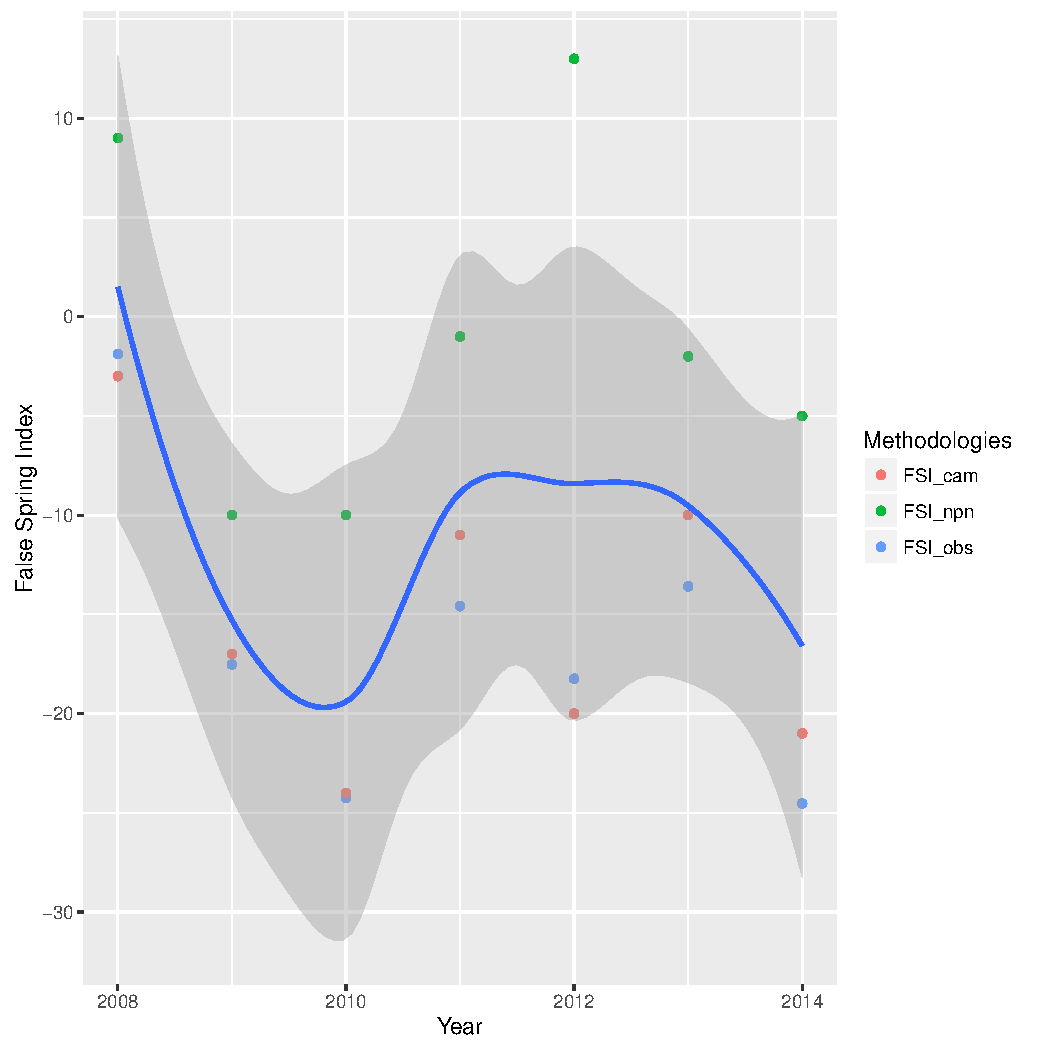
\includegraphics[width=\maxwidth]{figure/fsifig-1} \caption[A scatterplot indicating FSI values from 2008 to 2014 for each methdology used in this study]{A scatterplot indicating FSI values from 2008 to 2014 for each methdology used in this study. PhenoCam FSI values are red, Observed FSI values are blue, and USA-NPN FSI values are green.}\label{fig:fsifig}
\end{figure}




\section*{Supplement}
\begin{knitrout}
\definecolor{shadecolor}{rgb}{0.969, 0.969, 0.969}\color{fgcolor}\begin{kframe}
\begin{verbatim}
## lmer(formula = risk ~ chilling + warm + photo + (chilling + warm + 
##     photo | species), data = dxx)
##             coef.est coef.se
## (Intercept) 53.35     6.15  
## chilling    -0.10     0.36  
## warm        -1.54     0.19  
## photo       -1.19     0.15  
## 
## Error terms:
##  Groups   Name        Std.Dev. Corr              
##  species  (Intercept) 17.27                      
##           chilling     0.61    -0.73             
##           warm         0.50    -1.00  0.78       
##           photo        0.29    -0.98  0.84  0.99 
##  Residual              7.44                      
## ---
## number of obs: 996, groups: species, 9
## AIC = 6896.2, DIC = 6861.6
## deviance = 6863.9
\end{verbatim}
\end{kframe}
\end{knitrout}

\begin{figure} [H] 
\begin{center}
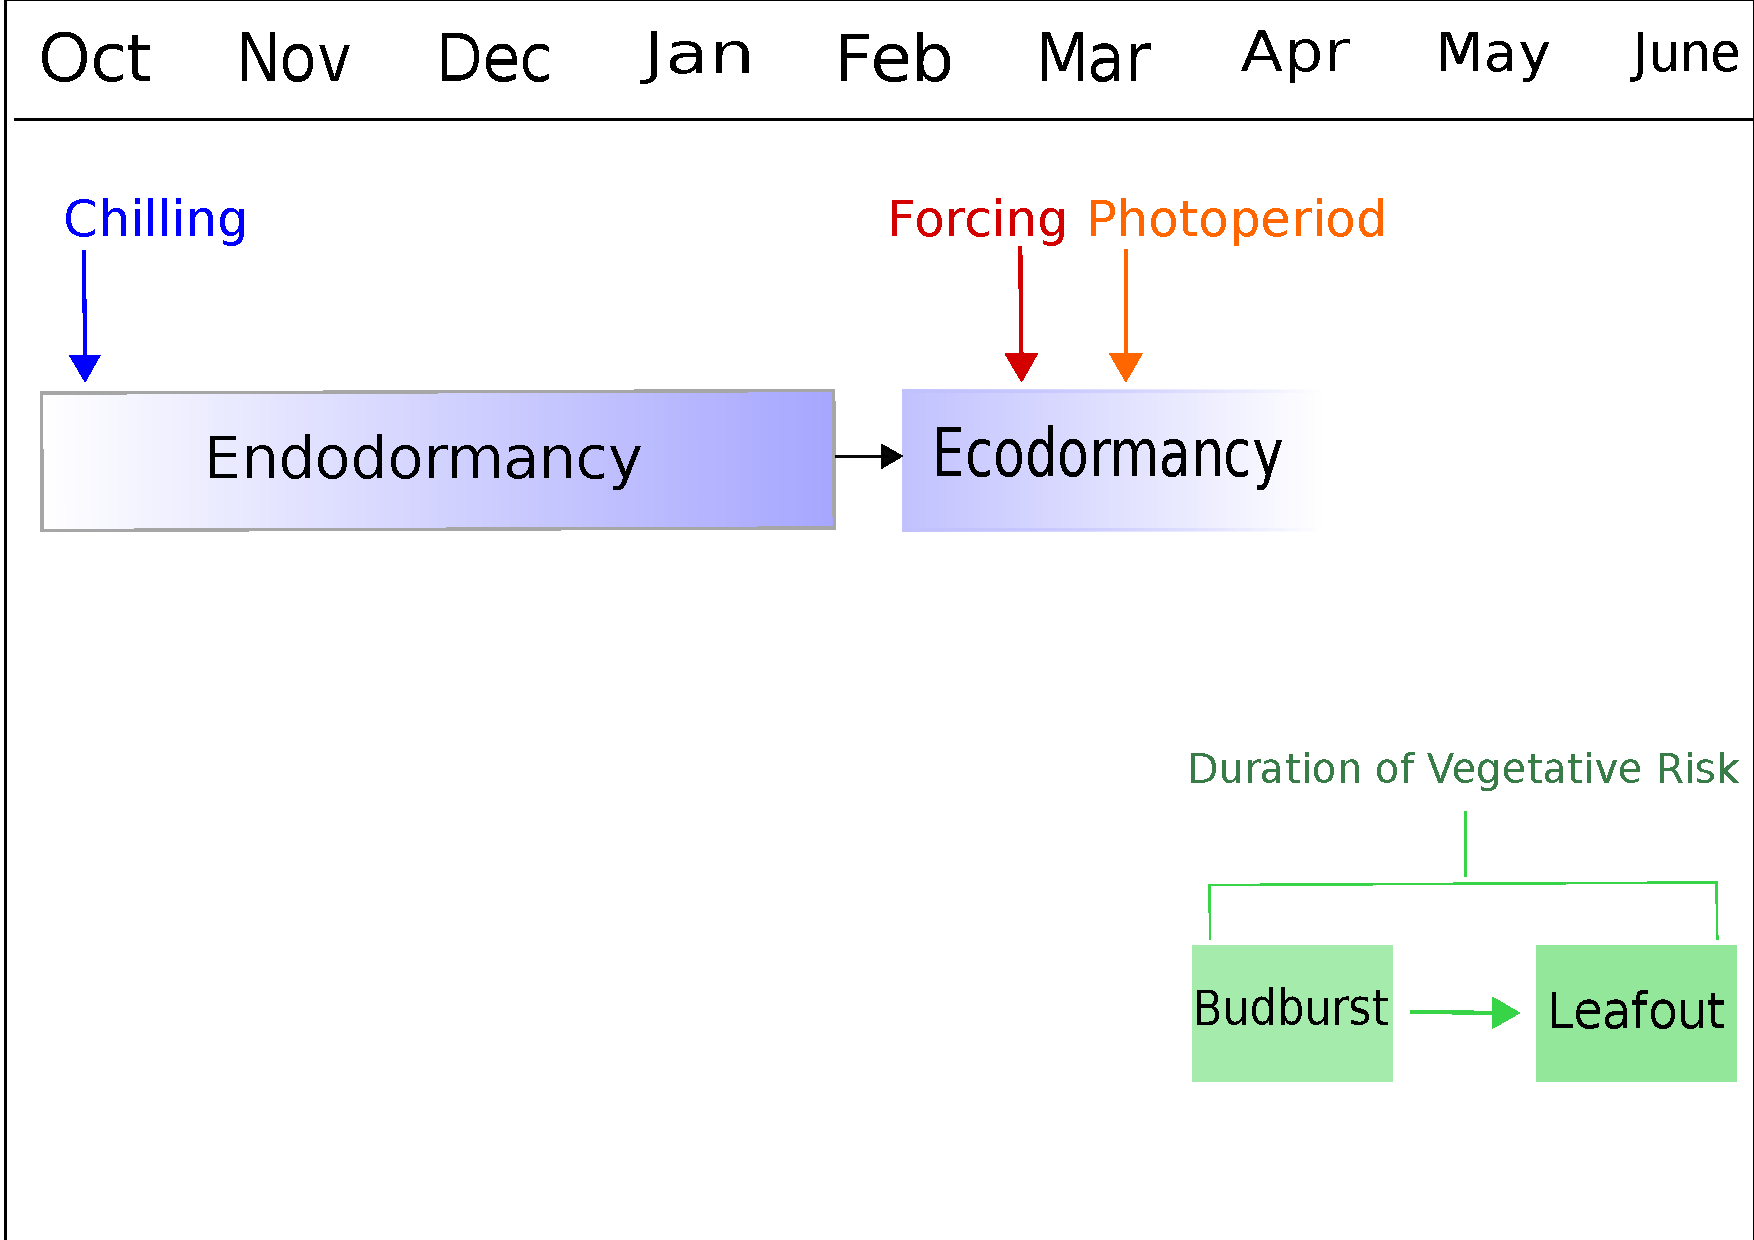
\includegraphics{..//figure/CuesAndFS.pdf}
\caption{Temperate forest trees utilize three main drivers to induce budburst in the spring: chilling over the winter, forcing temperatures in the spring, and longer photoperiod cues. During the endodormancy phase, individuals accumulate chilling hours and cannot break dormancy and false springs cannot occur during the this time. During the ecodormancy phase, however, false spring damage can occur. Damage from a false spring increases as the season progresses, however the likelihood of an event decreases.}\label{fig:cues}
\end{center}
\end{figure}

\begin{figure} [H] 
\begin{center}
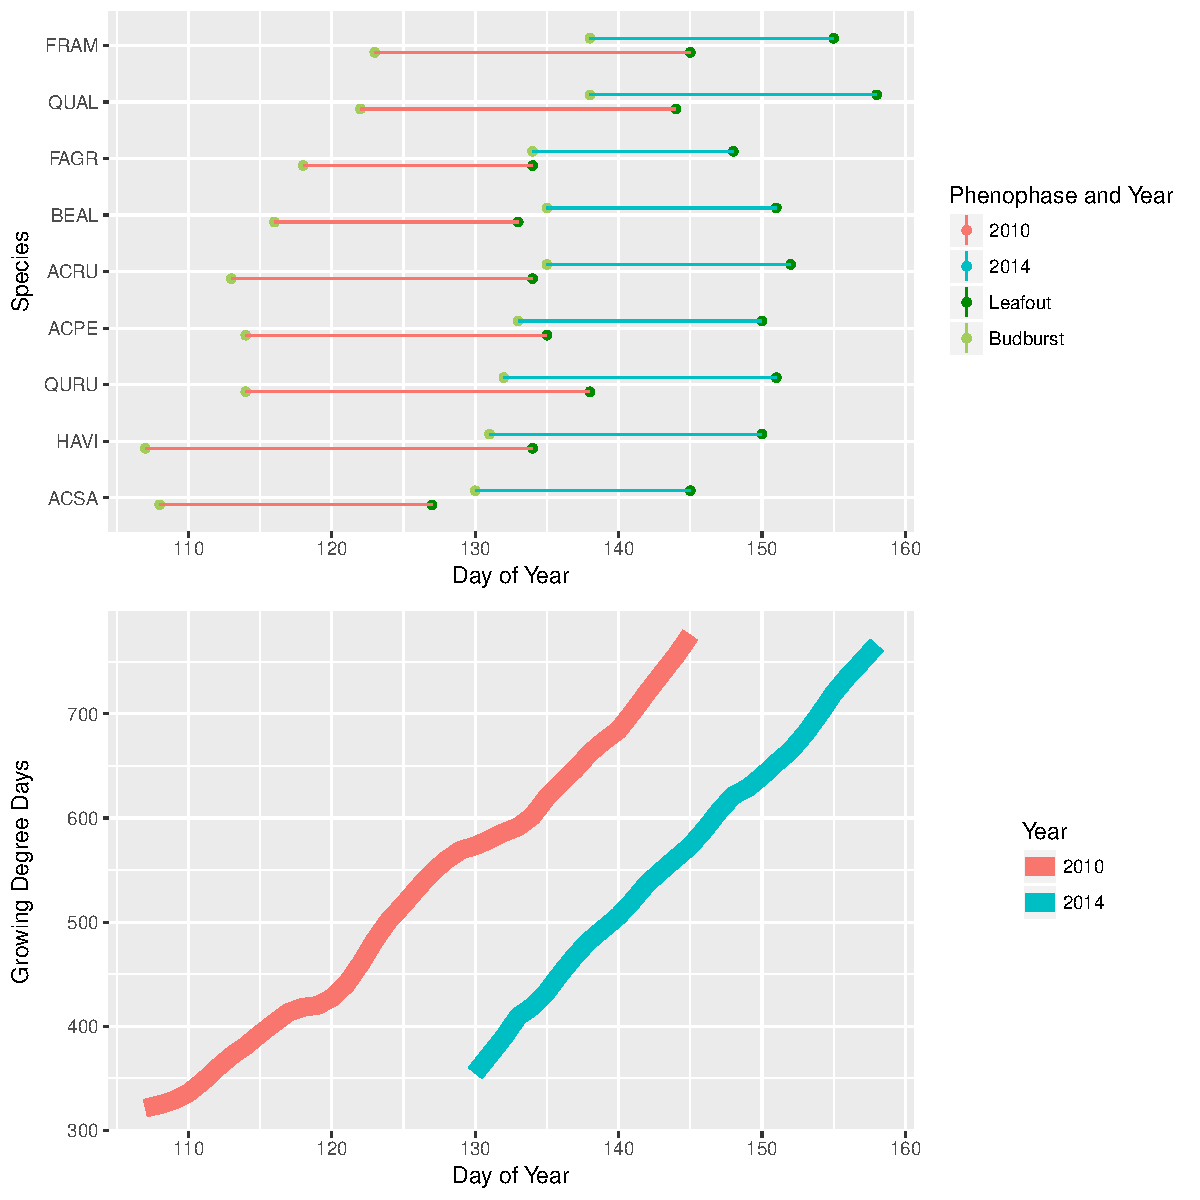
\includegraphics{..//figure/HF_gddTime.pdf}
\caption{A comparison of two years of observational data investigating the effects of growing degree days on the duration of vegetative risk. The average duration of vegetative risk for 2010 was 21 +/- 3.39 days versus 17.1 +/- 1.96 days in 2014.}\label{fig:forest}
\end{center}
\end{figure}

\begin{figure}[H]
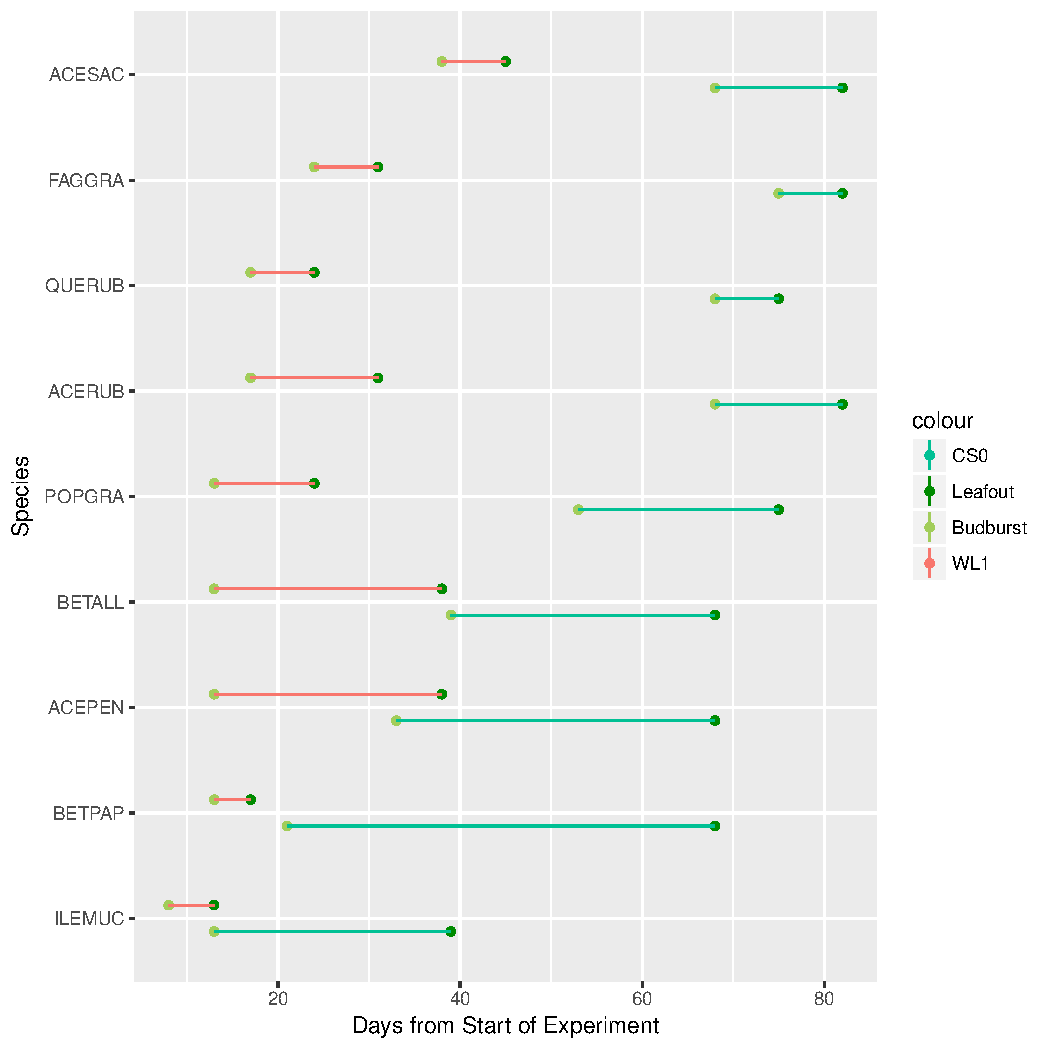
\includegraphics[width=\maxwidth]{figure/dan-1} \caption[Day of budburst and the day of leaf out for native tree species in New England]{Day of budburst and the day of leaf out for native tree species in New England. Data was collected from a growth chamber experiment using any combination of two photoperiod treatments, two forcing treatments, and three chilling treatments. The standard deviation is represented in blue for budburst and green for leaf out.}\label{fig:dan}
\end{figure}



\begin{landscape}
\begin{center}
\captionof{table}{Comparing damaging spring temperature thresholds in ecological and agronomical studies across various species and phenophases.} \label{tab:temperature} 
\footnotesize
\begin{tabular}{|c | c | c | c | c | c|}
\hline
\textbf{Sector} & \textbf{BBCH \citep{Meier2001}} & \textbf{Species} & \textbf{Temperature ($^{\circ}$C)} & \textbf{Type} & \textbf{Source} \\
\hline
Ecological & 9-15 & Sorbus aucuparia & -7.4 & 50\% lethality & \cite{Lenz2016} \\
\hline
Ecological & 9-15 & Prunus avium & -8.5 & 50\% lethality & \cite{Lenz2016} \\
\hline
Ecological & 9-15 & Tilia platyphyllos & -7.4 & 50\% lethality & \cite{Lenz2016} \\
\hline
Ecological & 9-15 & Acer pseudoplatanus & -6.7 & 50\% lethality & \cite{Lenz2016}\\
\hline
Ecological & 9-15 & Fagus sylvatica & -4.8 & 50\% lethality & \cite{Lenz2016}\\
\hline
Ecological & 9+ & All & -2.2 & hard & \cite{Schwartz1993}\\
\hline
Ecological & 9+ & All & -1.7 & soft & \cite{Augspurger2013} \\
\hline
Ecological & All & All & 2 SD below winter TAVG & cold-air outbreaks & \cite{Vavrus2006} \\
\hline
Ecological & 9+ & Eucalyptus pauciflora & -5.8 & elevated CO2 and temperature threshold & \cite{Barker2005} \\
\hline
Ecological & 9+ & All & -2.2 & 7 day threshold & \cite{Peterson2014} \\
\hline
Agrinomical & 9+ & All & 2 & Risk threshold for clear nights & \cite{Cannell1986} \\
\hline
Agrinomical & Floral & Vaccinium spp. & -4.4 to 0 & sprinkler protection threshold & \cite{Longstroth2012} \\
\hline
Agrinomical & 9 & Rosaceae & -7.2 & 10\% lethality & \cite{Longstroth2013}\\
\hline
Agrinomical & 9 & Rosaceae & -13.3 & 90\% lethality & \cite{Longstroth2013} \\
\hline
Agrinomical & All & All & Varies & Radiation Frost & \cite{Barlow2015} \\
\hline
Agrinomical & Floral & Wheat & -4 to -5 & 10-90\% lethality & \cite{Barlow2015} \\
\hline
Agrinomical & Vegetative & Wheat & -7 for 2hrs & 100\% lethality & \cite{Barlow2015} \\
\hline
Agrinomical & Vegetative & Rice & 4.7 & lethal limit & \cite{Sanchez2013} \\
\hline
Agrinomical & Vegetative & Corn & -1.8 & lethal limit & \cite{Sanchez2013}\\
\hline
Agrinomical & Vegetative & Wheat & -17.2 & lethal limit & \cite{Sanchez2013} \\
\hline
\end{tabular}
\end{center}
\end{landscape}
\restoregeometry

\begin{figure} [H] 
\begin{center}
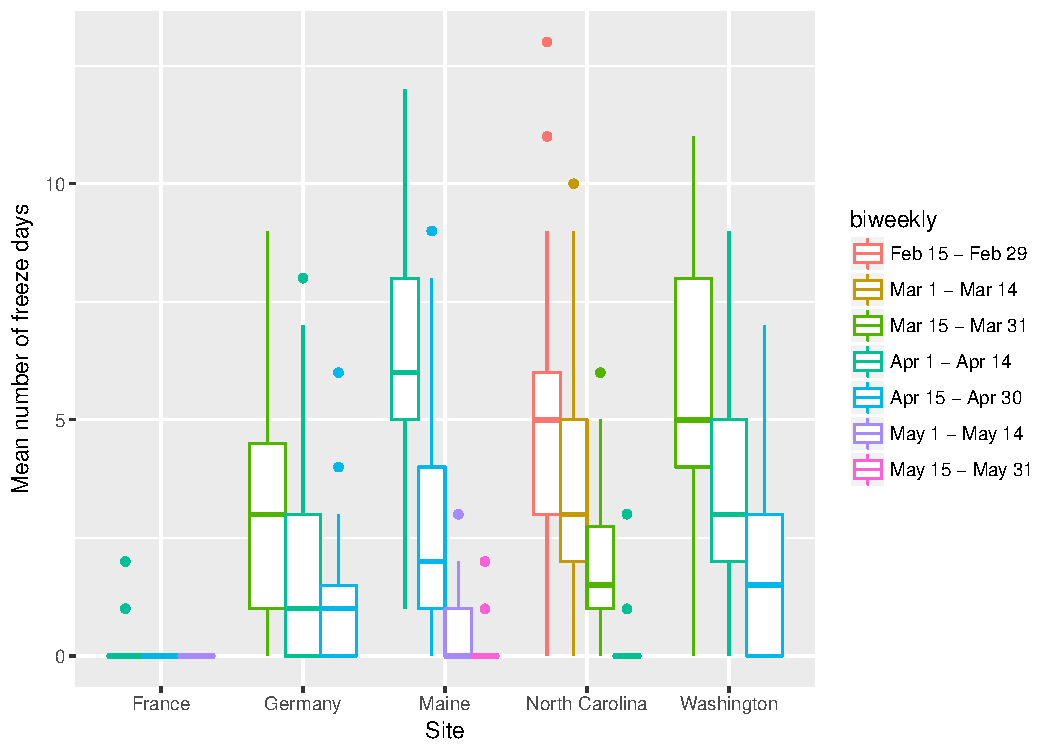
\includegraphics[width=16cm, height=13cm]{..//figure/Boxplot_RegRisk_biweekly.pdf} 
\caption{A comparison of false spring risk across five climate regions. The data was subsetted for each region based on earliest historical spring onset date to the latest historical leafout date and was divided into biweekly time periods \citep{Schaber2005, White2009, Soudani2012, USA-NPN2016}.}\label{fig:regional} 
\end{center}
\end{figure}

\end{document}
